\section{Module de croissance du zooplancton a deux proies}

\subsection{Description du module}

\begin{figure}
  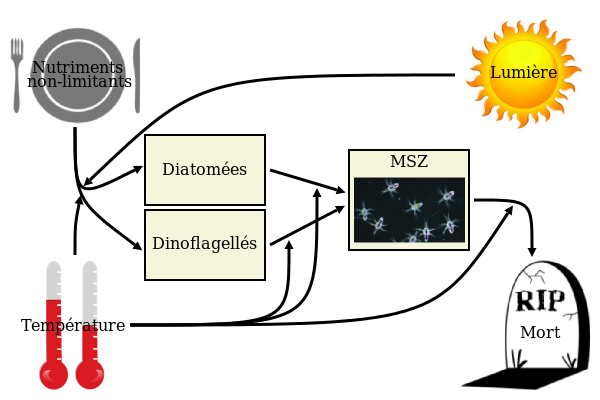
\includegraphics[width=\textwidth]{partie2/diagConc.png}
  \caption{Le modèle conceptuel du système étudié dans le cinquième cours. Par rapport
au modèle conceptuel du quatrième cours (voir figure~\ref{fig:partie1DiagConcept}) on
a augmonter les nombres des espèces (des diatomées et des dinoflagellés) qui peuvent
servir comme proie.
}
  \label{fig:partie2DiagConc}
\end{figure}

\begin{equation}
  {{d[DA]}\over{dt}} =
  \mu_{DA} [DA] - graz_{MSZ/DA} [MSZ]
  \label{eq:partie2DiffEq1}
\end{equation}
\begin{equation}
  {{d[DINO]}\over{dt}} =
  \mu_{DINO} [DINO] - graz_{MSZ/DINO} [MSZ]
  \label{eq:partie2DiffEq2}
\end{equation}
\begin{equation}
  {{d[MSZ]}\over{dt}} =
  \left (
    (1- eges_{MSZ}) graz_{MSZ} Y_{MSZ} - mm_{MSZ}
  \right ) [MSZ]
  \label{eq:partie2DiffEq3}
\end{equation}


\begin{equation}
  graz_{MSZ} = graz_{MSZ/DA} + graz_{MSZ/DINO}
  \label{eq:partie2grazMsz}
\end{equation}

\par{
Grazing non sélectif
}

\begin{equation}
  [PHYTO] = [DA] + [DINO]
  \label{eq:partie2nonSelEq1}
\end{equation}
\begin{equation}
  graz_{MSZ} = g_{MSZ} max(T) {{[PHYTO]^2}\over{kg_{MSZ}^2 + [PHYTO]^2}}
  \label{eq:partie2nonSelEq2}  
\end{equation}
\begin{equation}
  graz_{MSZ/DA} = graz_{MSZ} {{[DA]}\over{[PHYTO]}}
  \label{eq:partie2nonSelEq2}
\end{equation}
\begin{equation}
  graz_{MSZ/DINO} = graz_{MSZ} {{[DINO]}\over{[PHYTO]}}
  \label{eq:partie2nonSelEq3}
\end{equation}

\par{
Grazing sélectif
}

\begin{equation}
  graz_{MSZ/DA} = g_{MSZ} max(T) {{\left ( {{[DA]}\over{kg_{MSZ/DA}}}\right )^2}\over
{1 + \left ( {{[DA]}\over{kg_{MSZ/DA}}} \right )^2 + \left ( {{[DINO]}\over{kg_{MSZ/DINO}}} \right )^2}}
  \label{eq:partie2selEq1}
\end{equation}
\begin{equation}
  graz_{MSZ/DA} = g_{MSZ} max(T) {{\left ( {{[DINO]}\over{kg_{MSZ/DINO}}}\right )^2}\over
{1 + \left ( {{[DA]}\over{kg_{MSZ/DA}}} \right )^2 + \left ( {{[DINO]}\over{kg_{MSZ/DINO}}} \right )^2}}
  \label{eq:partie2selEq2}
\end{equation}
\begin{equation}
  graz_{MSZ} = g_{MSZ/DA} + g_{MSZ/DINO}
  \label{eq:partie2selEq3}
\end{equation}

\begin{table}
\begin{center}
\begin{tabular}{ | c | c | c | c | c | c | }
\hline
Variable & Reference & Test 1 & Test 2 & Test 3 & Test 4 \\
\hline
DA & $20$ & $30$ & $10$ & $20$ & $20$ \\
DINO & $20$ & $10$ & $30$ & $20$ & $20$ \\
MSZ & $10$ & $10$ & $10$ & $1$ & $20$ \\
\hline
\end{tabular}
\end{center}
  \caption{Les conditions initiales pour en DA, DINO et MSZ pour les tests different.}
  \label{tab:partie2params}
\end{table}

\subsection{Simulation de référence}

\begin{figure}
  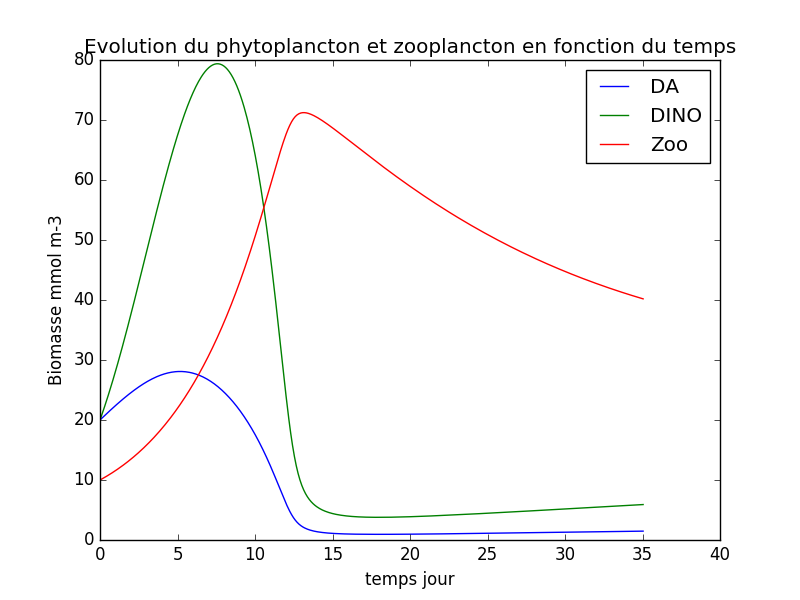
\includegraphics[width=.5\textwidth]{partie2/1Selec.png}\hfill
  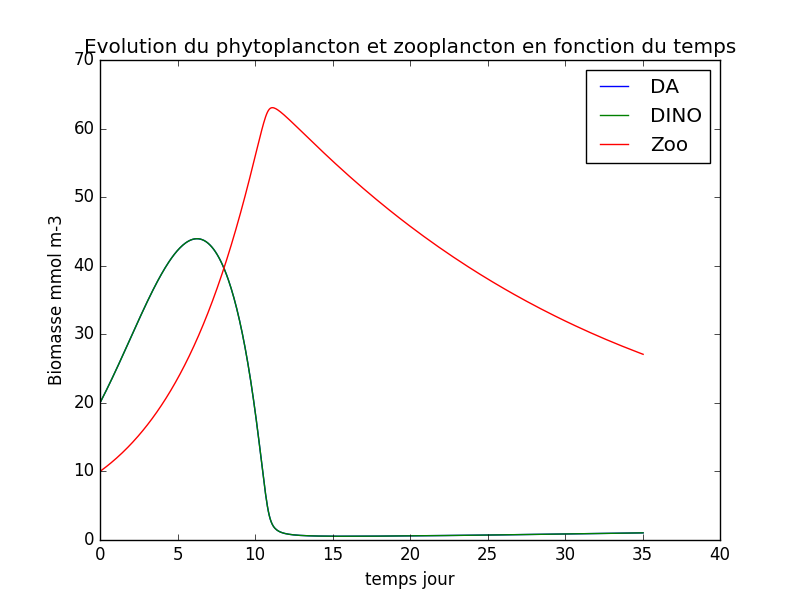
\includegraphics[width=.5\textwidth]{partie2/1Nonselec.png}
  \caption{Comparison 
Le graphe à droite montre \todo}
  \label{fig:partie2Ref}
\end{figure}

\subsection{Tests de la sensitivité}

\begin{figure}
  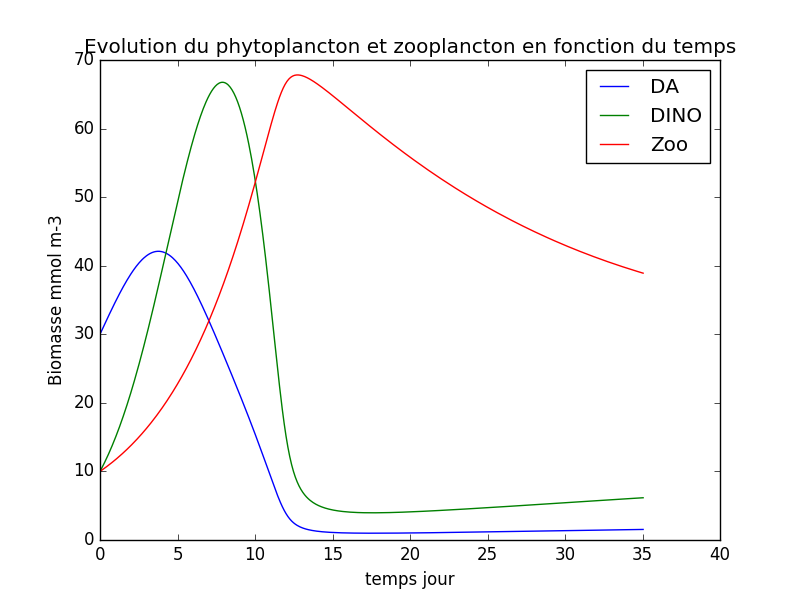
\includegraphics[width=.5\textwidth]{partie2/test1sel.png}\hfill
  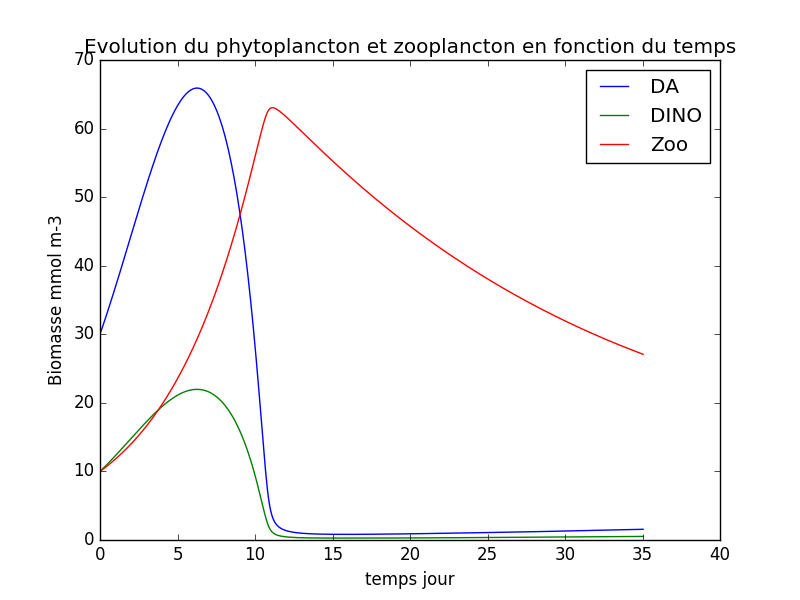
\includegraphics[width=.5\textwidth]{partie2/test1nonsel.png}\\
  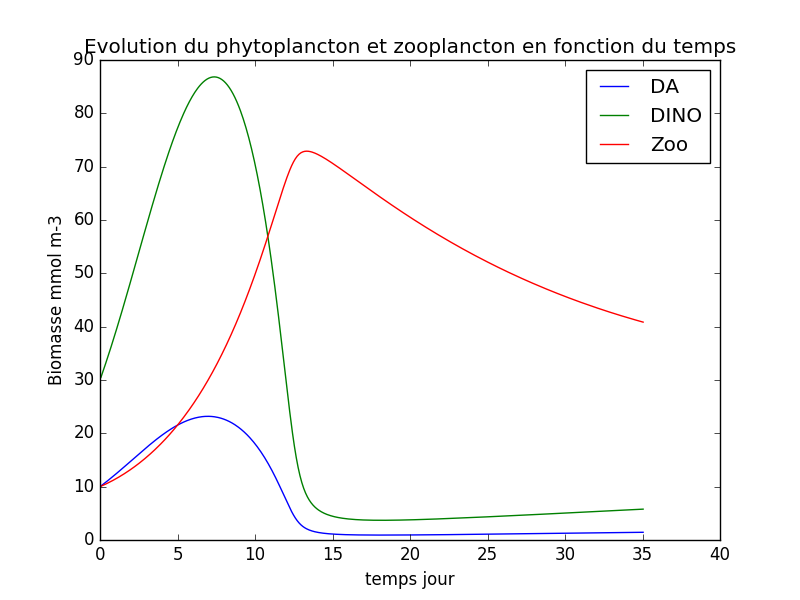
\includegraphics[width=.5\textwidth]{partie2/test2sel.png}\hfill
  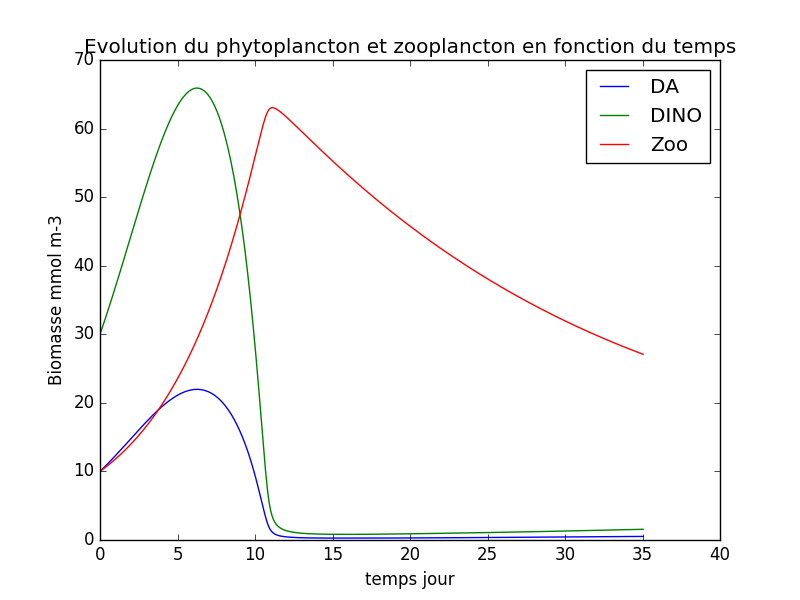
\includegraphics[width=.5\textwidth]{partie2/test2nonsel.png}
  \caption{\todo}
  \label{fig:partie2Test1}
\end{figure}
\begin{figure}
  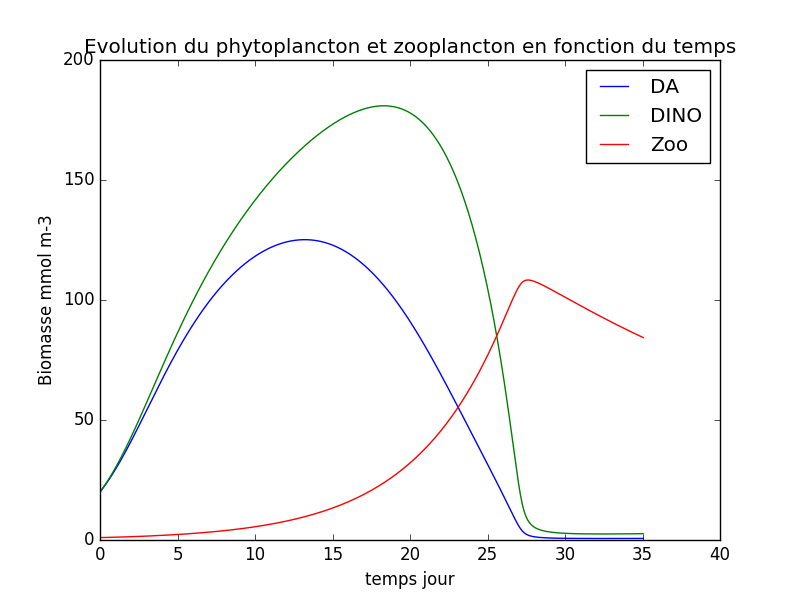
\includegraphics[width=.5\textwidth]{partie2/test3sel.png}\hfill
  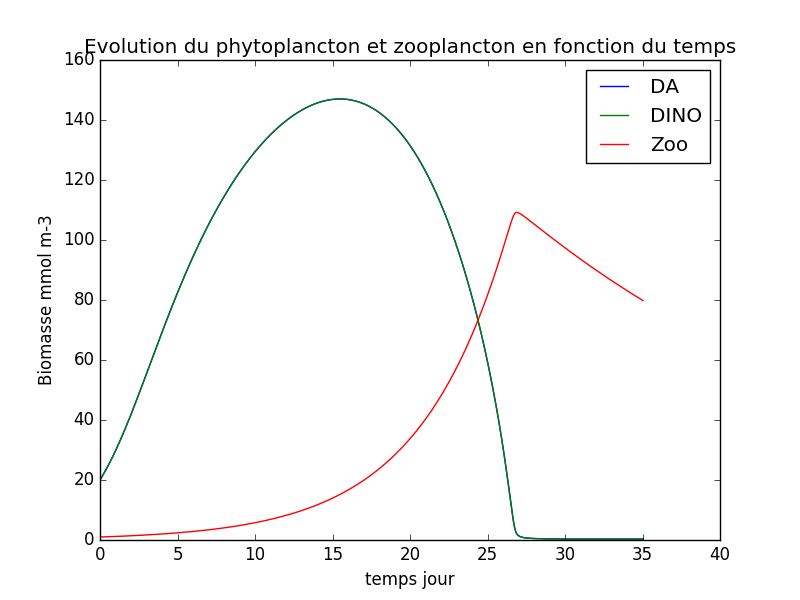
\includegraphics[width=.5\textwidth]{partie2/test3nonsel.png}\\
  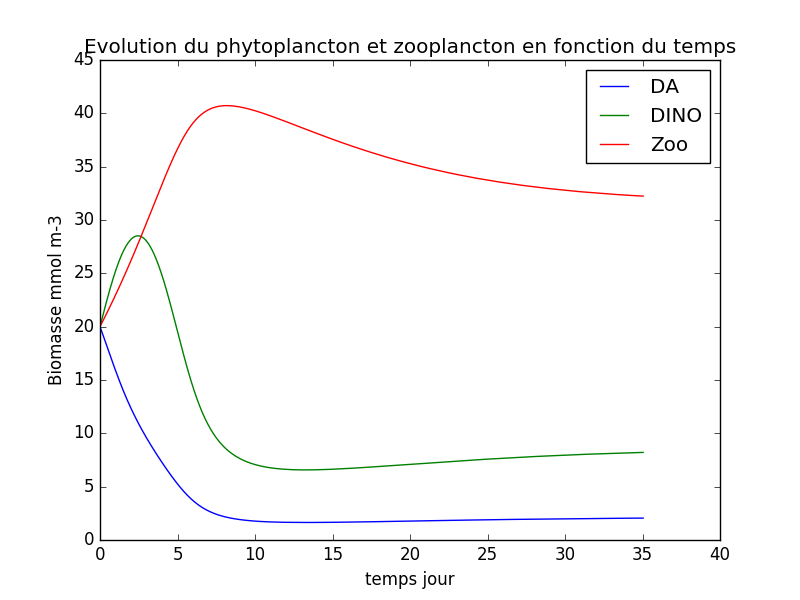
\includegraphics[width=.5\textwidth]{partie2/test4sel.png}\hfill
  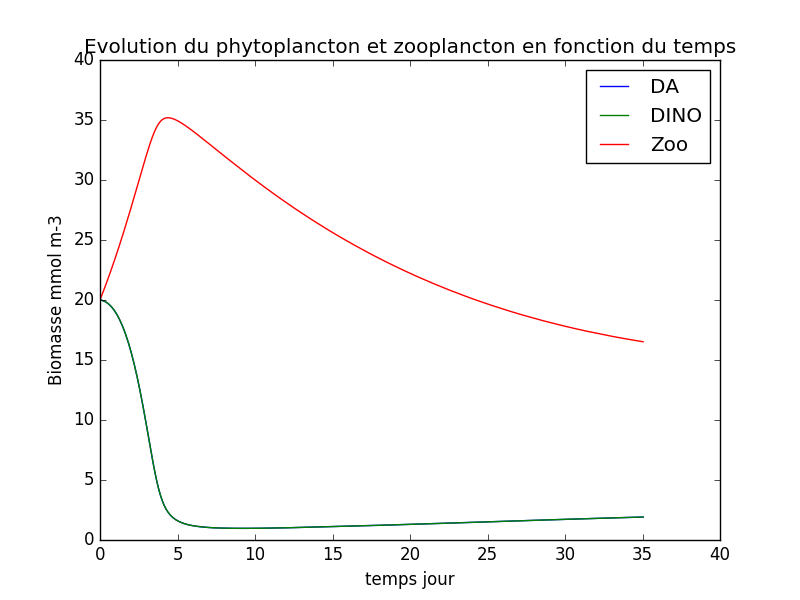
\includegraphics[width=.5\textwidth]{partie2/test4nonsel.png}
  \caption{\todo}
  \label{fig:partie2Test2}
\end{figure}

\subsection{Conclusion}

\par{
La proire(?) DINO a toujour plus de temps pour la croissance.
Dans le non-selective kg
Dans le selective on a un de kg qui est augmonter, le phyto peut plus croitre ...
quand kg moins
des resultats ``inverse''
Ca depends de la valeur de kg.
}
